%==============================================================================
% Teaching-mode example for the OSU / Soundbendor beamer style.
% Every style decision lives in sty/osu.sty; this file is content only.
% Build:  latexmk -pdf teaching.tex
% Handout (overlays flattened):  add "handout" to the \documentclass options.
%==============================================================================
\documentclass[10pt,aspectratio=169,xcolor=table]{beamer}
\usepackage[campus=cascades, mode=teaching]{sty/osu}

\title{Loops}
\course{CS 101}{Introduction to Computer Science}
\instructor{Prof.\ Benny Beaver}
\courseterm{Fall 2026}

\begin{document}
\maketitle

%------------------------------------------------------------------------------
\begin{frame}{Today}
  \begin{objectives}
    By the end of today you will be able to:
    \begin{itemize}
      \item write a \keyword{for} loop and a \keyword{while} loop
      \item state a \term{loop invariant}
      \item explain to a friend why your program is \emph{still running}
    \end{itemize}
  \end{objectives}
  \begin{aside}[Logistics]
    Homework 3 is due Friday. Homework 3 was also due last Friday.
    Homework 3 is, itself, a loop.
  \end{aside}
\end{frame}

%==============================================================================
\section{Doing Things Repeatedly}
%==============================================================================

\begin{frame}{Definitions}
  \begin{definition}[Loop]
    A \term{loop} repeats a block of code while a \keyword{condition} holds.
  \end{definition}
  \begin{definition}[Loop invariant]
    A \term{loop invariant} is a statement that is true before and after
    every iteration, much like your instructor's office hours: always
    \sout<2->{empty} \only<2->{\hl{lightly attended}}.
  \end{definition}
  \begin{example}
    While \var{coffee} $> 0$: grade one exam, then decrement \var{coffee}.
  \end{example}
  \begin{alertblock}{Warning}
    If \var{coffee} is never decremented, grading never ends.
    Ask any TA.
  \end{alertblock}
\end{frame}

\begin{frame}[fragile]{A First Loop}
  \begin{columns}[T]
    \column{0.5\textwidth}
      \begin{lstlisting}[style=numbered]
def count_sheep(n):
    """Fall asleep efficiently."""
    for i in range(n):
        print(f"{i+1} sheep")
    return "zzz"

count_sheep(3)
\end{lstlisting}
    \column{0.45\textwidth}
      \begin{itemize}
        \item<1-> \code{range(n)} yields $0, 1, \dots, n-1$
        \item<2-> The loop body runs \keyidea{exactly $n$ times}
        \item<3-> The \var{i} in \code{f"\{i+1\}"} is
                  \sym{off by one} on purpose
      \end{itemize}
      \medskip
      \begin{pitfall}<3->
        \code{range(1, n)} runs $n-1$ times. Your sheep will notice.
      \end{pitfall}
  \end{columns}
\end{frame}

\begin{frame}{Fill in the Blank}
  \begin{itemize}
    \item A loop that never stops is called an \blank<2->{infinite loop}.
    \item A loop inside a loop is called a \blank<3->{nested loop}.
    \item A loop that only runs on Mondays is called a \blank<4->{bug report}.
  \end{itemize}
  \bigskip
  \begin{funfact}<4->
    The first recorded infinite loop was a student asking
    ``will this be on the exam?''
  \end{funfact}
\end{frame}

%==============================================================================
\section{Check Your Understanding}
%==============================================================================

\begin{frame}{Clicker Question}
  \begin{quiz}
    How many times does \code{while x < 10: x += 0} run when \var{x} $= 0$?
    \begin{choices}
      \choice 0
      \choice 10
      \choice 11
      \correctchoice<2->{Yes}
    \end{choices}
  \end{quiz}
  \begin{answer}<2->
    It runs forever, so ``yes'' is the most honest answer.
    Partial credit for anyone who answered while it was still running.
  \end{answer}
\end{frame}

\begin{frame}{Think, Pair, Share}
  \begin{question}
    Is ``I will start the homework tomorrow'' a loop invariant?
  \end{question}
  \pause
  \begin{tryit}[Try It (2 minutes)]
    With a neighbor, write the loop that this sentence describes.
    Identify its termination condition, if any.
  \end{tryit}
  \pause
  \begin{takeaway}
    Every loop needs \keyidea{progress toward termination}.
    So does every homework.
  \end{takeaway}
\end{frame}

%==============================================================================
\section{Reasoning About Loops}
%==============================================================================

\begin{frame}{Pseudocode}
  \begin{columns}[T]
    \column{0.52\textwidth}
    \begin{algorithm}[H]
      \caption{FindMax}
      \Input{list $A$ of $n$ snacks, ranked by tastiness}
      \Output{the tastiest snack}
      \BlankLine
      $m \gets A[1]$\;
      \For{$i \gets 2$ \KwTo $n$}{
        \tcp{invariant: $m = \max(A[1..i-1])$}
        \If{$A[i] > m$}{
          $m \gets A[i]$\;
        }
      }
      \KwRet{$m$}\;
    \end{algorithm}
    \column{0.44\textwidth}
      \begin{enumerate}
        \item<1-> \textbf{Initialization}: true before the loop
        \item<2-> \textbf{Maintenance}: each step keeps it true
        \item<3-> \textbf{Termination}: at the end, $m = \max(A)$
      \end{enumerate}
      \medskip
      \uncover<3->{Formally, \(m = \argmaxl_{a \in A}\ \text{tastiness}(a)\).}
  \end{columns}
\end{frame}

\begin{frame}{A Note on Simplification}
  Students sometimes ``simplify'' like this:
  \[
    \frac{\sin x}{n} \;=\; \frac{\mathrm{si}\cancel{\mathrm{n}}\,x}{\cancel{n}}
      \;=\; \mathrm{six} \;=\; 6
  \]
  \pause
  \begin{pitfall}
    Cancellation applies to \stress{factors}, not to letters that look alike.
    The same applies to loop indices \var{i} and \var{l}, and to the
    numeral \code{1}.
  \end{pitfall}
\end{frame}

%==============================================================================
\section{Reference Material}
%==============================================================================

\begin{frame}{Lists}
  \begin{columns}[T]
    \column{0.32\textwidth}
      Default:
      \begin{enumerate}
        \item Write loop
        \item Run loop
        \item Wait
      \end{enumerate}
      \medskip
      Mini-template \code{[a)]}:
      \begin{enumerate}[a)]
        \item Panic
        \item Add print
        \item Find bug
      \end{enumerate}
    \column{0.32\textwidth}
      \begin{itemize}
        \item Loops
          \begin{itemize}
            \item \code{for}
              \begin{itemize}
                \item over a range
                \item over a list
              \end{itemize}
            \item \code{while}
          \end{itemize}
        \item Recursion
          \begin{itemize}
            \item see: Recursion
          \end{itemize}
      \end{itemize}
    \column{0.32\textwidth}
      \begin{description}
        \item[break] leave the loop
        \item[continue] skip ahead
        \item[pass] do nothing, enthusiastically
      \end{description}
  \end{columns}
\end{frame}

\begin{frame}{Tables and Figures}
  \begin{columns}[T]
    \column{0.42\textwidth}
      \centering
      \rowcolors{2}{beaver!12}{white}
      \begin{tabular}{rr}
        \rowcolor{beaver!90}
        \textcolor{white}{$\mathbf{n}$} & \textcolor{white}{$\mathbf{n!}$} \\
        1 & 1 \\ 2 & 2 \\ 3 & 6 \\ 4 & 24 \\ 5 & 120 \\ 6 & 720 \\
        7 & 5{,}040 \\ 8 & 40{,}320 \\
      \end{tabular}
      \captionof{table}{Factorials, computed with a loop.}
    \column{0.54\textwidth}
      \begin{figure}
        \begin{subfigure}{0.48\linewidth}
          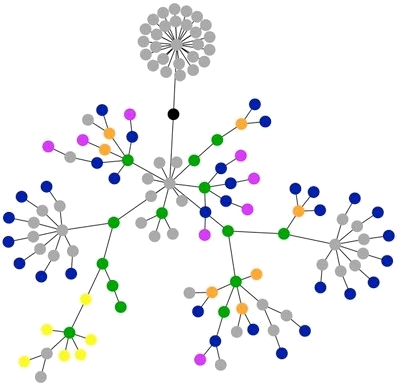
\includegraphics[width=\linewidth]{img/graphic}
          \caption{Iteration 1}
        \end{subfigure}\hfill
        \begin{subfigure}{0.48\linewidth}
          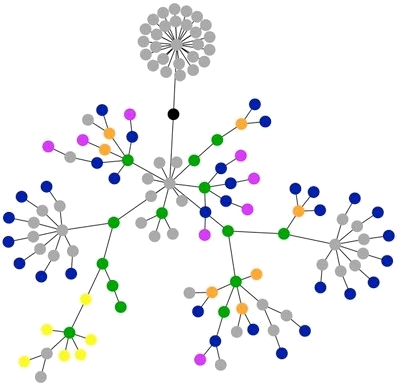
\includegraphics[width=\linewidth]{img/graphic}
          \caption{Iteration 2}
        \end{subfigure}
        \caption{The loop made no visible progress. Suspicious.}
      \end{figure}
  \end{columns}
\end{frame}

\begin{frame}{Loop Invariants: The Song}
  \begin{columns}[T]
    \column{0.3\textwidth}
      \href{http://www.haverford.edu/computerscience/resources/songs/}{\textbf{Loop Invariants}}\\
      by \textit{J.\,P. Dougherty}\par\medskip
      \mediabutton{media/loop-invariants.mp3}{Play}
      \par\medskip
      {\scriptsize\color{crater} Opens in your system's audio player.}
    \column{0.33\textwidth}
      \footnotesize\itshape
      Loop invariants, loop invariants\\
      Keep me on the road,\\
      Loop invariants, loop invariants\\
      As I write my code.\par\medskip
      Preconditions, postconditions,\\
      Help to shed some light.\\
      Assertions used to write the loop\\
      Will help me get it right.
    \column{0.33\textwidth}
      \footnotesize\itshape
      Loop invariants, loop invariants\\
      They can be a pain.\\
      Loop invariants, loop invariants\\
      Oh, but what I gain.\par\medskip
      Executing, substituting,\\
      Each does complement.\\
      Code correctness is the goal\\
      Of loop invariants.
  \end{columns}
\end{frame}

\begin{frame}{Highlighting Cheat Sheet}
  \small
  \begin{tabular}{@{}lll@{}}
    \toprule
    \textbf{Command} & \textbf{Looks like} & \textbf{Use for} \\
    \midrule
    \code{\textbackslash term}    & \term{loop invariant} & a term being defined \\
    \code{\textbackslash keyword} & \keyword{iteration}   & technical vocabulary \\
    \code{\textbackslash keyidea} & \keyidea{always terminate} & the one idea to remember \\
    \code{\textbackslash var}     & \var{count}           & a variable in prose \\
    \code{\textbackslash sym}     & \sym{$\neg$, $\wedge$} & symbols, operators \\
    \code{\textbackslash mat}     & \mat{$\mathbf{W}$}    & matrices, tensors \\
    \code{\textbackslash stress}  & \stress{never}        & spoken emphasis \\
    \code{\textbackslash code}    & \code{while True}     & inline code \\
    \code{\textbackslash hl}      & \hl{read this}        & highlighter \\
    \code{\textbackslash badge}   & \badge{new} \badge[pinestand]{easy} & tags \\
    \bottomrule
  \end{tabular}
\end{frame}

\begin{frame}{OSU Colors}
  \centering\osupalette
\end{frame}

\begin{frame}{One Deck, Two Modes}
  Shared slides can adapt to the mode:
  \begin{itemize}
    \item \teachingonly{This line only appears in \textbf{teaching} mode.}%
          \researchonly{This line only appears in \textbf{research} mode.}
    \item Switch with \code{mode=research} or \code{mode=teaching}
    \item Switch campus with \code{campus=corvallis} or \code{campus=cascades}
  \end{itemize}
\end{frame}

\begin{frame}[standout]
  Questions?\\[0.5em]
  {\normalsize (Office hours: the loop that never terminates.)}
\end{frame}

{%
  \setbeamercolor{background canvas}{bg=white}
  \begin{frame}[plain]
    \centering\vfill
    This is a blank frame: no title bar, no logos, no page number.\\
    Good for a full-screen image (\code{\textbackslash fullbleed\{img/photo\}}) or a dramatic pause.
    \vfill
  \end{frame}
}

\end{document}
